\documentclass[10pt, a4]{article}
\usepackage{natbib}
\bibliographystyle{apalike}
\usepackage{geometry}
\usepackage{lineno}
\usepackage{mathrsfs}

\usepackage{amsmath,amssymb}
\usepackage{graphicx}
\usepackage[linesnumbered, ruled]{algorithm2e}
\linespread{1.3}

\newcommand{\beginsupplement}{%
        \setcounter{table}{0}
        \renewcommand{\thetable}{S\arabic{table}}%
        \setcounter{figure}{0}
        \renewcommand{\thefigure}{S\arabic{figure}}%
     }

\usepackage{titling}
\title{Agemo: an open-source library for Laplace transformed coalescence time distributions.}
\author{Gertjan Bisschop \thanks{g.bisschop@sms.ed.ac.uk} \\ Institute of Evolutionary Biology, University of Edinburgh, EH9 3FL Edinburgh, Scotland}
\date{}

%%%
\pretitle{\begin{flushright}\LARGE} % makes document title flush right
\posttitle{\end{flushright}}
\preauthor{\begin{flushright}\large} % makes author flush right
\postauthor{\end{flushright}}
\predate{\begin{flushright}\large} % makes date title flush right
\postdate{\end{flushright}}

\begin{document}

\maketitle

%%ABSTRACT
\section*{Abstract} %this is the popgroup abstract needs to be improved
%central point: importance of the GF approach, and why a lack of speed currently lets the approach down
%we can use phase information now: huge step forward preparing us for the fully phased era.
\texttt{agemo} is an open-source tool with a python API that allows users to generate the Laplace transform of the coalescence time distribution of a sample under any structured coalescent model. In addition, \texttt{agemo} provides ways to efficiently query that distribution, by using the fact that its generating function can be represented most simply as a directed graph with all possible ancestral states of the sample as nodes. Past implementations have not made full use of this, relying on computer algebra systems instead of graph traversal to process these recursive expressions.
\texttt{agemo} can be used to compute the probabilities of the joint site frequency spectrum for blocks of a given size, under the specified model. Calculating these probabilities requires repeated differentiation of the generating function which suffers from an explosion in the number of terms when implemented naively. Using a closed-form expression for the coefficients of a series expansion of the equations associated with each edge, we can efficiently propagate these coefficients through the graph avoiding redundant operations.

\vspace{0.25cm} 
\linenumbers

%%INTRODUCTION
\section{Introduction}

Laplace transforms have been used extensively in coalescent theory since the introduction of the structured coalescent \citep{Takahata1988, Notohara1990, Barton1995}. Initially it was a formal tool to analyse continuous-time Markov chains \citep{Takahata1988, Griffiths1991, Wilkinson-herbots1998}. But as noted by \citet{Wilkinson-herbots1998}, the Laplace transforms of the distributions of coalescence times are also interesting in their own right. The Laplace transform of a random variable has a clear probabilistic interpretation. One can think of that random variable as describing the length of an interval. If a Poisson marking process with intensity $\omega$ marks the interval, then the Laplace transform $f^*(\omega)$ is the probability of not observing any marks in the considered interval \citep{Rade1972}. Let the random variable be the stochastic process modelling the (sum of the) exponentially distributed waiting times describing the ancestry of a random sample, then the marking process can describe the arrival of mutations. Formulated as such, the connection to the coalescent \citep{Kingman1982, Hudson1983, Tajima1983} becomes obvious, making the Laplace transform a natural choice \citep{Weissman2017}.

Moreover, used in mathematical fields like queueing theory, the Laplace transform often provides us with an alternative description of the behaviour of a system, often simplifying its analysis in the process. In essence, this is what the generating function (GF) method as described in \citet{Lohse2011} does. Using the probabilistic interpretation of the Laplace and the fact that the transform turns convolution into multiplication (see \ref{GF_description}), one can come up with a much simpler, recursive and automated, description of the distribution of the (sum of) inter-event times given a set of samples and a (structured coalescent) model. Phrased differently, being given a flow diagram or coalescent state space graph describing all possible transitions during the coalescent process (see fig. \ref{fig:graph}), one can readily write down all associated expressions in the Laplace domain. This is not the case for the time domain.\\

The GF framework has been used to tackle two major problems in population genetics: estimating sweep parameters \citep{Bisschop2021} as well fitting explicit models of population history \citep{Lohse2011, Bunnefeld2015, Lohse2016}. To study the how fast populations diverge in the face of gene flow, a lot of focus has gone to isolation with migration type (IM) models \citep{Nielsen2001}. This class of models where two populations split off from an ancestral population at some point in the past and experience gene flow between them from that point onwards are simple yet informative. They allow us to study the impact of ongoing gene flow on the coalescent histories along the genome. It has been remarked before that the GF framework is general in the sense that most of the analytical results for specific instances of these types models are just special cases of the general solution provided by the GF \citep{Lohse2016}. %this section needs work

The ability to make mathematically tractable descriptions of a problem as well the ability to efficiently implement the solution are two bottlenecks that hold for all inference problems (in population genetics). The first issue is generally solved by making simplifying assumptions about recombination, either ignoring the information contained within closely linked variants completely \citep{Gutenkunst2009, Excoffier2013}, or by only ignoring recombination within very short blocks \citep{Yang2002, Hey2004, Lohse2011}. Additionally, because the state space of all possible events describing the coalescent history of a sample will grow super-exponentially with sample-size and the number of considered events, there will always be limitations to the sample size and/or the number of events for which a detailed description of the ancestral process can be generated and more importantly evaluated within reasonable (memory) space and time.

The second issue is often very closely connected to the type of mathematical description used. In general, one will benefit from the potential to implement a particular solution in terms of data structures for which efficient algorithms exist for each of the required basic operations. For example, preserving matrix structure up to the point of evaluation, as used in phase-type theory \citep{Hobolth2019}, will tend to have a positive impact on performance due to the existence of many efficient algorithms for linear algebra operations.

So far, all inference approaches using the GF, rely on deriving the probability of observing each of the different block-wise site frequency spectrum (bSFS) vectors. These combinations of mutation configurations along the distinguished branch types within blocks of a certain length summarise the joint distribution of linked polymorphisms \citep{Bunnefeld2015}. However, depending on both the number of observed mutations and the number of distinguished branch types, they require repeated differentiation of the entire GF. As a consequence, any naive implementation of the GF with higher-order derivatives using a computer algebra system (CAS) will quickly run into computational bottlenecks, essentially limiting the extendability of the framework.

Previous efforts to make the framework more efficient have targeted the first bottleneck category by limiting the number of distinguishable branch types, limiting the number of occurrences of particular events, and using symmetries within the recursive description \citep{Lohse2016}. No attempts have been made to tackle the second bottleneck and describe the problem in a way that allows for more efficient computation.\\

Here we present the first open-source implementation of the GF framework and lay out the key algorithms that allow us to efficiently calculate the bSFS by using the correspondence between the recursive formulation of the Laplace transform and the coalescent state space graph. The focus on the bSFS is only superficial however. Any future extension of the library will make use of the concepts outlined here.

First, we will outline how the GF can be represented more succinctly. Secondly, we will lay out the graph traversal algorithm allowing us to efficiently evaluate the GF. We will then apply this to the bSFS by using the algorithm to propagate the coefficients of a truncated Taylor series through the graph. Finally, we show how to extend bSFS type calculations to the fully phased and rooted case by making use of mutation type symmetries to limit the amount of computation needed.

%%SECTION LT as array and paths
\section{Methods}
\subsection{Recursive description of the Laplace transform} \label{GF_description}
%this section should make everything about the Laplace transform clear such that it is obvious to understand in the next section what the equations look like, and what the dummy variables associated with branch types do and mean.
\subsubsection{single population}

Given a sample of $n$ uniquely labelled lineages $\Omega = \{a, ..., n\}$ coming from a single population, we can represent all possible coalescent histories of that sample as a series of trees. In each of these ranked topologies nodes represent the lineage ancestral to the subtended nodes. Alternatively, the same information can be captured by a single rooted directed graph describing the state space of all (coalescence) events affecting the history of the sampled lineages. In this graph, each node is uniquely labelled by one of the partitions of $\Omega$. As lineages coalesce, we move through the graph from the source node, representing the set of all sampled lineages, to the root or most recent common ancestor (mrca). In the case of the neutral coalescent and a single population each path through the graph is equivalent to a single ranked topology. However, in general the state space graph will contain information on all events that affect the lineage configuration, not only those that join to lineages. %last sentence should be better. Or perhaps only mention this in the next section (general form).

For $k$ uncoalesced lineages, the rate of coalescence is ${k}\choose{2}$ (in units of $2N_e$ generations). Because each step is conditionally independent of the previous and as touched upon in the introduction, the Laplace transform of the sum of inter-event times or the time to the most recent common ancestor ($t_{mrca}$) is a simple product of all Laplace transforms of the random variable describing the waiting time to go from $k$ to $k-1$ lineages. As such, we can associate each edge of the directed graph with a single equation describing this transition. The Laplace transform of the $t_{mrca}$ for a single (ranked) topology can then be retrieved by multiplying the equations associated with a single path of the graph. Likewise, the entire GF is the sum of all expressions retrieved by a depth-first traversal of the graph (see \ref{fig:graph}). %

%what a SINGLE EQUATION will look like
Knowing that the equation associated with a single edge in the coalescent state space graph as outlined above, gives the probability of observing the coalescence event prior to any other event happening at rate $\omega$, for any two out of $k$ lineages, the Laplace transform is $f^{*}(\omega) = \frac{1}{{k\choose{2}} + \omega}$. Note that in general we can label each branch connecting two lineages in a coalescent tree by the samples that will be affected by a mutation arising during the time represented by that branch. And in general, we will associated each of these branch types with a unique dummy variable. Replacing $\omega$ by $\sum_{i=1}^{b} \omega_i$, we can retrieve the coalescence time distribution for each of the $b$ distinguished branch types \citep{Lohse2011}. 

%extend to MULTIPLE EVENTS
%%stress fact that here coalescent trees and state space graph start to diverge, events are included in the graph!!
\subsubsection{general form}
So far, we have dealt with a single population, tracking only coalescence events. In a structured population, we require at least one type of (migration) event to ensure lineages eventually all end up in the same population to allow for coalescence. These events can be incorporated in the state space graph by adding a node for each of these events and labelling that node by their impact on the tracked set of lineages. Looking at any node in the graph, the set of all possible events is determined by all outgoing edges and the set of all observable branchtypes during the time represented by each edge will be given by the label of the node from which the edges are leaving. The LT associated with a single edge still describes the probability of observing a particular event prior to all other events. So as long as the events that we have added in are associated with exponentially distributed waiting times and given that $min(X, Y) \sim exp(\omega_1+\omega_2)$ when both $X \sim exp(\omega_1)$ and $Y \sim exp(\omega_2)$, we can still readily associate each edge with the correct equation.

%%EQ_GENERAL_FORM_LT
\begin{equation} \label{eq:general_form}
f[\boldsymbol{\omega}] = \frac{c}{\sum c_i\kappa_i + \sum l_j\lambda_j + \sum o_k \omega_k} 
\end{equation}

Here, Roman letters represent integers counting the number of ways a certain (coalescence or other) event can take place ($c_i, l_j$) given the current state space, or the number of branches of a particular type ($o_i$). The Greek letters represent the rate of the associated competing processes. Note that in the case of coalescence with multiple populations, rates are relative and given by $\kappa_i = N_{e_{i}}/N_{e_{ref}}$.

Each equation can be encoded as a matrix with two rows containing the integer coefficients ($c$, $c_i, l_j, o_k$). The first row represents the numerator and will only contain a single non-zero value. The second row then represents the denominator. Storing the equations this way ensures we can efficiently substitute in parameter values by taking the dot product with a vector representing a point in parameter space ($\kappa_i, \lambda_j, \omega_k$) once the Laplace transform needs to be evaluated. Also, storing equation coefficients in array form allows us to efficiently perform operations on the equations (see \ref{discrete_events}). A minimal representation of the GF therefore consists of an array containing all unique equations, and an array of arrays with equation indices describing all paths through the graph. 

%%FIG:GRAPH
\begin{figure}
\begin{center}
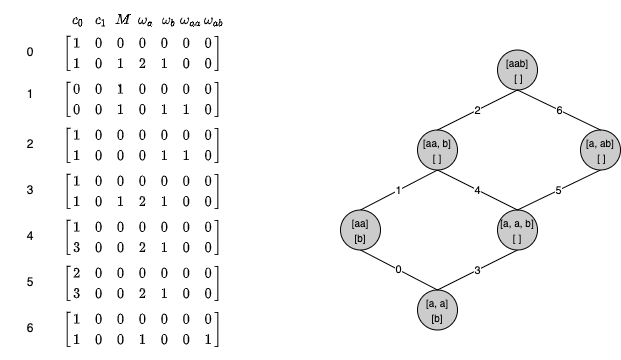
\includegraphics[scale=0.5]{figures/temp2b.png} \label{fig:graph}
\end{center}
%caption
\caption{\textbf{From coalescent state space to equation array:} coalescent state space graph for two populations $A$ and $B$ with 2 and 1 unphased sample(s) respectively. The demographic model assumes a single mass migration event from population $B$ to $A$ back in time.}
\end{figure}

\subsubsection{discrete events} \label{discrete_events}

For the general description of the GF we have assumed that all competing processes have exponentially distributed waiting times. It is possible however to incorporate events that only happen once. Initially treating these discrete events as a competing exponential process with rate $\delta$, we can recover the GF parametrised by the discrete time $T$ of the event, by taking the inverse transform of the GF divided by its associated dummy variable ($\delta$). This has been used to incorporate population splits and bottlenecks \citep{Lohse2011, Bunnefeld2015} as well as hard sweeps \citep{Bisschop2021}.

Previous implementations have relied on a CAS to get an analytic solution for the inverse transform upon each evaluation of the GF. However, it is clearly overkill to determine the inverse Laplace symbolically repeatedly given that the GF will always be a sum of products of factors of the form $c/(d+\delta)$ with $c$ and $d$ constants, independent of the complexity of the state space graph. That is, at least as long as we limit ourselves to a single discrete event. Having stored all equation coefficients as an array, we can formulate a closed-form solution to the inverse Laplace that allows for efficient substitution of all parameter values (see \ref{eq:inverse_laplace}). 

If we want to maintain the outlined correspondence between the state space graph and the GF as a sum of the products of the expressions associated with each path then we have to modify the state space graph. This can be done by creating a new node for each section of all paths leading up to a node associated with a discrete event. Each of these new nodes is connected to the root of the graph by a single edge associated with its respective inverse (see fig. \ \ref{fig:equation_graph}).

In essence this means that the part of the path downstream of the discrete event remains unaltered, each edge still associated with a simple equation of the form \ref{eq:general_form}. While each path upstream of that node is now collapsed into a single node. Once this operation has been performed, each path of the graph represents a product of factors again. Under the hood however, we perform a graph inversion while collapsing turning edges into nodes and vice versa (see fig. \ \ref{fig:equation_graph} C). This simplifies the graph traversal algorithm (see \ref{graph_traversal}). 

%%FIG:EQUATION_GRAPH
\begin{figure}
\begin{center}
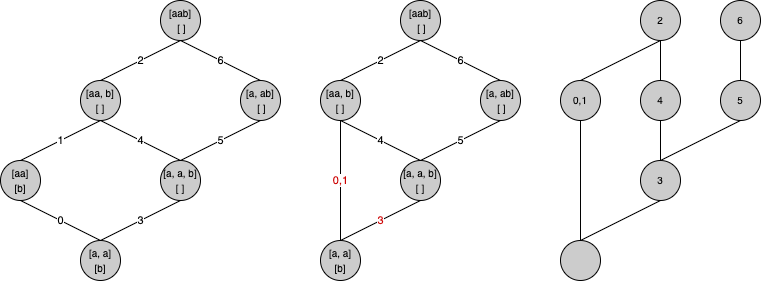
\includegraphics[scale=0.5]{figures/temp3.png}\label{fig:equation_graph}
\end{center}
%caption
\caption{\textbf{From coalescent state space to equation graph:} setup identical as fig.\ \ref{fig:graph}. A shows the initial coalescent state space graph, while B shows the collapsed form grouping all parts of each path that require inverting with respect to the dummy variable associated with the discrete event. C takes this logic one step further turning the (sets of) equations previously associated with the edges into nodes, simplifying algorithms that do not require state space information.}
\end{figure}

\subsubsection{adding new events}

Currently, besides coalescence, two types of events have been implemented: uni-directional migration at a constant rate and population splits (forwards in time). Other events can readily be incorporated by adding in a method that provides a description of what the event does to the configuration of lineages (or node label) while generating the state space graph. There are two limitations however. First of all, the defined events should not lead to cycles in the directed graph. For example, in line with \citet{Lohse2016} migration is limited to being uni-directional such that lineages cannot cycle indefinitely between populations without ever reaching the fully coalesced state. Finally, note that so far our approach is only compatible with a single discrete event. Adding in more discrete events would require the use of a CAS to determine the inverse transform.

%%%GRAPH TRAVERSAL
\subsection{graph traversal} \label{graph_traversal}

Given an equation graph (as described in \ref{discrete_events}) and a dependency sequence describing the evaluation order of the graph, a general algorithm to propagate any evaluation of the equations associated with each node is given by alg.\ \ref{alg:propagation}. It relies on the fact that implicitly the edges of the graph represent multiplication. Once both multiplication and addition have been defined for the propagated values we can rely on the commutative property to efficiently traverse the graph towards the root. Especially in the case where addition is a less costly operation than multiplication (as is the case for polynomials, see \ref{bsfs}), it will pay off to add the values associated with the children of a node prior to multiplication. We can now apply this algorithm to efficiently calculate the bSFS. 

%%ALG PROPAGATION	
\begin{algorithm}\label{alg:propagation}
    \SetKwInOut{Input}{Input}
    %\SetKwInOut{Output}{Output}
	
    \underline{function PROPAGATE}\;
    \Input{adjacency list of graph, node\_values, evaluation\_order}
    
    \ForEach{parent in evaluation\_order}{
    	children = graph[parent]\;
    	temp = 0\;
    	\If{children}{
    \ForEach{child in children}{
    temp+=node\_values[child]\;
    }
    \eIf{parent not root}{node\_values[parent] = PRODUCT(temp, node\_values[parent])\;}
   {\Return{temp\;}}
    }
     		}

    \caption{Propagate values through graph.}
\end{algorithm}

\subsection{blockwise site frequency spectrum} \label{bsfs}

\subsubsection{graph traversal}
The block-wise site frequency spectrum or bSFS is the vector of site frequency spectrum counts in short blocks of a fixed length \citep{Bunnefeld2015}. It is the probability of seeing $k_i$ mutations on each of the $i$ distinguished branchtypes. For an unphased sample of size 3 the bSFS would be a vector of the form $\{k_1, k_2\}$ with $k_1$ and $k_2$ representing the number of singletons and doubletons respectively. Each count is an element within the interval $[0, 1, 2, ... , k_i^{max} + 1]$ where $k_i^{max} + 1$ is used to bin all mutation configurations with more than $k_i^{max}$ mutations. 

Deriving the probability for each of the $(\prod_{i=1}^{c} k_i^{max} + 2)$ possible bSFS configurations, with $c$ the length of the bSFS vector, has thus far been the way in which the recursively generated Laplace transform of coalescence time distributions has been used. The probability of observing mutation configuration $\boldsymbol{k}$ under a specified model can be obtained by taking the $k_i \textsuperscript{th}$ derivative with respect to $\omega_i$ (see eq.\ (1) in \citet{Lohse2011} for details).

Any naive approach, based on calculating all higher order derivatives using a CAS, will suffer from an explosion in the number of terms due to the Leibniz or product rule when differentiating. Generally a CAS will fail to take into account the fact that the same partial derivatives are computed multiple times. This problem has been well-studied for the purpose of automatic differentiation algorithms \citep{Neidinger1992, Neidinger1995, Griewank2000, Bettencourt2019}. One possible approach to overcome this issue consists of implementing recurrence relations on how to build and combine the coefficients of truncated Taylor series. For such a series, the coefficient of $x^\bold{k}$ is indeed proportionate to the desired partial derivative. By defining the series coefficients for all elementary functions and defining the recurrence relations for arithmetic operators as well as function compositions one can build higher-order derivatives from the ground up while avoiding having to recalculate the same derivative multiple times\citep{Neidinger2013}.

Translating this to the graph traversal algorithm outlined above requires us to first obtain all coefficients for a truncated Taylor series of the equation associated with each node in the equation graph. We can then use the algorithm defining the product of two truncated Taylor series (see alg.\ (8) in \citet{Neidinger2013} and alg.\ \ref{alg:product}) to propagate the coefficients of the series associated with each node. Note that adding two truncated Taylor series simply amounts to the pairwise addition of all corresponding coefficients. To get at the higher order derivatives needed for the first step, we could use the recurrence relations as defined in \citet{Neidinger2013}. However, all equations associated with each of the nodes of the equation graph are well characterised. They fall into one of two categories depending on wether an inversion step was needed. For each of the two categories we can define a closed-form implementation of the derivatives with respect to the distinguished branchtypes (see eqs.\ \ref{eq:deriv_polynomial} and \ref{eq:deriv_exponential}). 

%%PRODUCT
\begin{algorithm}\label{alg:product}
    \SetKwInOut{Input}{Input}
    \SetKwInOut{Output}{Output}

    \underline{function SERIES\_PRODUCT}\;
    \Input{Two same-size arrays of floats $a$ and $b$}
    \Output{array $c$ of same size as $a$ and $b$}
    \ForEach{multi-index $\boldsymbol{k}$}{
    	$sum = 0$\;
        \ForEach{multi-index $\boldsymbol{j} \leq$ multi-index $\boldsymbol{k}$}{
           
            sum = ADD(sum, $a[\boldsymbol{j}] * b[\boldsymbol{k}-\boldsymbol{j}])$\;
        }
        $c[\boldsymbol{k}]=$ sum\;
        }
    \Return $c$[ ]\;
    \caption{Product of two truncated Taylor series \citep{Neidinger2013}.}
\end{algorithm}

%potential floating point precision issues
Remark that alg.\ \ref{alg:product} contains an explicit \texttt{ADD} function. Care needs to be taken when summing (a subset of) the coefficients of a Taylor series. These will be both positive and negative, and as such catastrophic cancellation might occur leading to accuracy loss. The compensated summation algorithm of Ogita-Rump-Oishi \citep{Ogita2005} is implemented as an efficient way to bound the potential loss in accuracy. Another way of handling this would be to temporarily increase numeric precision at the crucial steps. Lastly, an advantage of using Taylor series coefficients rather than the derivatives is that the coefficients will always be smaller by a factor $(\sum \boldsymbol{k})!$ leading to less cumulative roundoff error.


\subsubsection{Mutation type equivalences} %make sure language usage concerning mutation configurations/mutation types is always the same.

When labelling each branch by the labels of the lineages it subtends, the number of branch types and therefor the number of mutation types (a single bSFS vector), will quickly go up. Calculating the probability for observing each one of these will become unfeasible very fast. To alleviate this we can make two types of simplifications. Following \citet{Lohse2016}, we can remove phase and/or root information by a relabelling of the branches. This reduces the number of branch types and mutation types one distinguishes. Phase is removed by labelling all branches according to their number of descendants in each subpopulation. Root information on the other hand can be left out by consistently labelling each branch by the set of lineages it subtends or by the complement of that set. Note that applying these simplifications might mean one cannot fully use all information present in a dataset.

Additionally, we can make use of the fact that some mutation types are inherently equiprobable. For example, given a sample from a single population labelled $\{\{a, b, c\}\}$ mutation type $\{a, ab\}$ will have the same probability as 5 other mutation types. To determine this equivalence it suffices to see that each mutation type can be represented in two ways. Either each mutation type is labelled as an integer vector indicating presence or absence of one or more mutations along branch types $\{a, b, c, ab, ac, bc\}$. In our example this equates to $\{1, 0, 0,1, 0, 0\}$. We can apply a similar representation rule to all branch types as well resulting in in a boolean vector containing 1's for the samples the branch subtends. Because each mutation type consist of no, one or multiple branch type(s), a single matrix combining the vectors for the branch types present can represent a mutation type as well. For this representation, all permutations of columns representing samples from the same population represent equiprobable configurations.

Besides all this, a large fraction of mutation types is simply impossible to observe. Realising that the bSFS is a sparse array can reduce computation time even further by limiting computation to those mutation types that can actually be observed.

\section{Results and Discussion}

The work presented here constitutes a CAS-independent, open-source implementation of the GF approach. A general outline has been given on how to rely on the correspondence between the coalescent state space graph and the GF to query the distribution of Laplace transformed coalescence times efficiently. In particular, an algorithm has been laid out to efficiently calculate the bSFS making this package ideal as a backend for likelihood calculations. To quantify the speedup of the new algorithm we compare its performance against the original implementation \citep{Lohse2011} as well as against a simulation-based approach as described in \citet{Beeravolu2018}. Using \texttt{msprime} \citep{Baumdicker2021} coalescent trees can be simulated under (almost) any demographic model. Without having to simulate mutations we can calculate the probability for each of the distinguished mutation types. Given that mutations on each branch type happen independently, the probability of seeing mutation configuration $(k_1, k_2, ..., k_n)$ is given by the product of $n$ probabilities as given by a Poisson distribution with rate $\theta * t_i$. Here, $t_i$ is the branch length of branch type $i$ and $\theta=2N_e\mu$. When averaged across many replicates the true value will be approximated. Note that particular entries of the bSFS might require fewer/more replicates to get at a good approximation than others \citep{Beeravolu2018}.  
%in Beervolu et al. : for IM-type model with 1000 replicates one can already approach the true bSFS quite well. But, would be good to have a measure that tells us to stop simulating rather than simply having to pick an arbitrary value. 
Fig \ref{fig:comparison} shows ... %explain timing results here. Would it be worth adding memory requirements as well?\\ 

%presented algorithm is limited to including a single discrete event. This is not a huge limitation in the sense that CAS would also struggle with performing multiple inverse Laplace transforms for the equations associated with the GF.
%There might be a point whenever one might want to analyse more complex models (e.g.\ containing more than one discrete event) that the need for relying on symbolic algebra or automatic differentiation becomes necessary. 
%This does not change the general idea outlined in this paper. It will still pay off to evaluate the building block equations associated with the coalescent state space graph first, and then rely on graph traversal to get to the correct results. This could be achieved by putting in place a function to propagate a user-provided array (with first dimension equal to the number of equation nodes) through the graph using user-defined addition and multiplication rules. This way, we would not have the additional burden of having a CAS as a direct dependency. %confusing!


%section on potential improvements; moving part of code to C, other algorithms to multiply polynomials, ...
Currently, \texttt{agemo} is implemented in \texttt{python 3}, relying on \texttt{numba} just-in-time compilation to speed up the critical parts of the code. Compiling the code using \texttt{numba} has a few consequences. Firstly, compilation happens each time the code is run and will require a few seconds. This is generally not an issue given that usually for a single model many points in parameter space will be evaluated. Secondly, some numerical operations are implemented differently in \texttt{numba} than in \texttt{numpy}. This is particularly true for summation and has required us to implement a compensated sum algorithm. A potentially faster solution would be to temporarily increase machine precision for the evaluation of particular sums. This is not possible using \texttt{numba} however and would require us to transfer part of the code to \texttt{C}. 

There are more efficient algorithms to multiply (truncated) multivariate polynomials. The fast Fourier transform (FFT) would allow us to perform the operation at $\mathcal{O}(n log(n))$ with $n$ the order of the polynomial instead of $\mathcal{O}(n^2)$ for the current multiplication. However, gains would only be noticeable for a large number of distinguished branch types, or a really large $k_{max}$ value. 
\newline


%future extensions
incorporate more demographic events (bottleneck, mass migration events) and incorporate hard sweep approximations \citep{Bisschop2021}.
%input tree
Although most people still process vcfs when it comes to mutation data. There is the more succinct treesequence format containing both topology information as well as mutations. It would therefore make a lot of sense to add on the ability to calculate the likelihood of a mutation configuration under a particular coalescent model as given by a marginal tree from a treesequence. This boils down to restricting the GF for that particular model to the observed topology, counting the number of mutations of each distinguished branch type and computing its probability.
%potential issues: non resolved polytomies: option, let them correspond with multiple topologies rather than a single one.

%make link with MAGIC: deriving Laplacce transformed coalescence time distribution for empirical sequence data. Much easier to fit models

%section to end with:
%from increase in model complexity/sample size and impact on timing. It should become clear that ...
%as Laplace transform coalescence time distribution much easier to work with and to develop algorithms for. This paper paves the way for future work departing from these ideas.

These algorithms will not suddenly make it possible to extent the usage of the GF to any arbitrary model and sample size. The fact remains that the number of sample configurations grows superexponentially with sample size \citep{Lohse2016}. At some point complex models will be easier to simulate (and extract bSFS from) rather than use agemo. To what extent have we changed this point. Time of evaluation vs graph complexity. %model simplicity does not always need to be a burden.

\section*{acknowledgements}
This work was supported by an ERC starting grant (ModelGenomLand, 757648)

\bibliography{../../Latex/Bibliography/library}
\beginsupplement
\newpage
\section*{Supplementary Information}
\setcounter{equation}{0}
\setcounter{figure}{0}
\setcounter{table}{0}
\setcounter{page}{1}
\makeatletter
\renewcommand{\theequation}{S\arabic{equation}}
\renewcommand{\thefigure}{S\arabic{figure}}
\renewcommand{\bibnumfmt}[1]{[S#1]}
\renewcommand{\citenumfont}[1]{S#1}

\subsection*{closed-form derivatives}
%%DERIVATIVES POLYNOMIAL
%as formula
Given a first degree multivariate polynomial of the form $f(\bold{x}) = \sum c_ix_i + b$, then the following higher order derivatives have a closed form. With and $s = \sum k_i$

\begin{equation} \label{eq:deriv_polynomial}
\frac{\partial f(\bold{x})^{-1}}{\partial^{k_i} x_i} = (-1)^s s! \frac{c^{k_i}_i}{f(\bold{x})^2}
\end{equation}
%%DERIVATIVES EXPONENTIAL
%
\begin{equation} \label{eq:deriv_exponential}
\frac{\partial e^{c f(\bold{x})}}{\partial^{k_i} x_i} = c^sc_i^{k_i}e^{cf(\bold{x})}	
\end{equation}
These two base case derivatives together with the defined Taylor series product allow us to calculate all required derivatives for the entire GF assuming at most only a single inverse Laplace with respect to a discrete event is required.

\subsection*{closed-form inverse Laplace transform}
%%INVERSE LAPLACE
Given $f(c) = \frac{1}{c+\delta}$, the inverse Laplace transforms (wrt $\delta$) can be defined as follows. Here $T$ represents the time to the discrete event.

\begin{equation} \label{eq:inverse_laplace}
g(T) = \mathscr{L}^{-1}(\frac{1}{\prod_{i=0} f_i(\bold{x})}) = \sum_i \frac{(-1)^{i+1} e^{-cT}}{\prod_{i\neq j} (f_{min(i,j)}(\bold{x})-f_{max(i,j)}(\bold{x}))}
\end{equation}

Note that all derivatives of \ref{eq:inverse_laplace} can be determined using the equations from the section above.


\end{document}
